\documentclass{article}

%\usepackage[left=2.5cm,right=2.5cm,top=1.5cm,bottom=1.5cm]{geometry}
\usepackage{anysize}
\usepackage{graphicx}
\usepackage{ngerman}
\usepackage{parskip}
\usepackage{amsmath, amsthm, amssymb, amsfonts}
\begin{document}

\section*{Verdichtermodellierung}
Das Kennfeld ist abhängig von diversen Konstanten und vom
augenblicklichen Vordruck.

$\pi$ ist das Verhältnis aus Hinterdruck und Vordruck, im Kennfelddiagramm (siehe Abb. \ref{fig:kf})
also eine konstante Funktion von $\varphi$.
\begin{equation}
\pi:=\frac{p_{\text{out}}}{p_{\text{in}}}
\label{eq:pi}
\end{equation}

Der Dispatcher-Agent darf sich wünschen, ob der Verdichter $V$ aktiv ist
oder nicht. Dem Wunsch auf Inaktivität wird immer entsprochen, dem auf
Aktivität nicht.

Der Arbeitspunkt $A$ eines aktiven Verdichters liegt immer im Kennfeld $K$
und immer auf $\pi$. Falls diese beiden Menge disjunkt sind, so ist der
Verdichter inaktiv.

Der Wunsch auf Aktivität muss immer mit einer Wunschleistung $W$ verbunden
sein. $W$ liegt zwischen 0\% und 100\% und wird vom Simulator auf eine
Leistung $L$ im Kennfelddiagramm umgerechnet.

Es gibt immer einen Schnittpunkt $S$ von $L$ und $\pi$. Liegt S in K, so ist $A = S$.

Liegt $S$ nicht in $K$, so ist $S$ der nächstgelegene Randpunkt von $K$, der auf
$\pi$ liegt. Per Konstruktion muss es einen solchen Punkt geben.

Oder anders gesagt:
\begin{itemize}
\item Bilde $D$ als Schnittstrecke von $\pi$ und $K$.
\item Bilde $S$ als Schnittpunkt von $\pi$ und $L$
\item Dann ist $A$ der $S$ nächstgelegene Punkt aus $D$.
\end{itemize}

\begin{figure}[!ht]
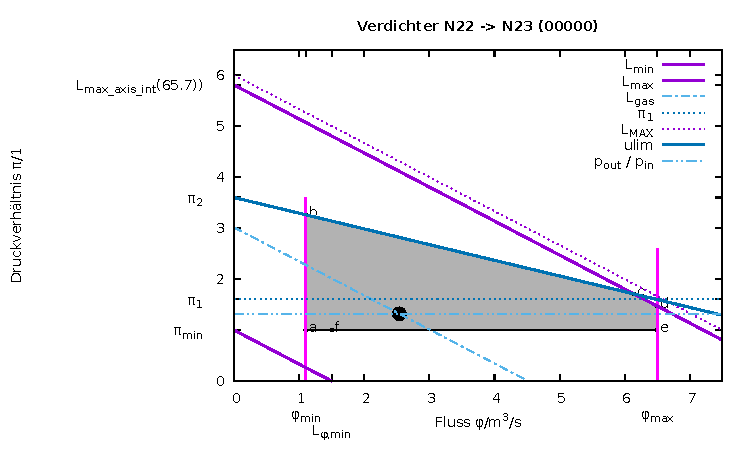
\includegraphics[width=0.9\textwidth]{Example_Compressor_Wheel_Map.pdf}
\caption{Verdichterkennfeld bla blubb}
\label{fig:kf}
\end{figure}
\end{document}
